\chapter{6}
\label{ch:6}

\todo{Name chapter}

\section{Methodology}

For this experiment, we used the same arXiv corpus analyzed in Chapters 4 and 5. To determine whether a URI links to an open access dataset or software resource, we used a hybrid classifier proposed in by Salsabil et al. \cite{salsabil2022study} for each article in the corpus. The classifier transforms each article into a text file using the PDFMiner\footnote{https://pypi.org/project/pdfminer/} Python library. By employing a regular expression, it scans the text to identify and extract sentences that contain URIs. Given the extracted sentences, the hybrid classifier combines two approaches: a heuristic classifier and a learning-based classifier. The heuristic classifier removes URIs that fall into two categories: those belonging to 54 major publishers such as Springer, Wiley, and Sagepub, and those that end with ``.pdf''. This is because publisher URIs are typically not associated with datasets or software repositories, and .pdf files are typically not datasets or software. The learning-based classifier was trained on a dataset of labeled sentences that contain URIs. The labeled samples were classified as either open access datasets/software (OADS), or not (non-OADS) as shown in Table \ref{tab:classifier}. The learning-based classifier used this information to learn how to classify new URIs. In the study by Salsabil et al., they found that the hybrid classifier is more accurate than either the heuristic classifier or the learning-based classifier alone. This is because the heuristic classifier eliminates many irrelevant URIs, and the learning-based classifier is able to accurately classify the remaining URIs.

\begin{table}
    \centering
    \begin{tabular}{|l|c|}
    \hline
    Sentences containing the URI & Category \\
    \hline
    The dataset is available at \url{http://ibm.biz/multishapeinsertion} & OADS \\
    \hline
    \begin{tabular}[c]{@{}l@{}}Code and materials for reproducing the experiment as well\\as all data and analysis scripts are open and available \\at \url{https://github.com/hawkrobe/pragmatics\_of\_perspective\_taking}.\end{tabular} & OADS \\
    \hline
    \begin{tabular}[c]{@{}l@{}}This article is available from: \\ \url{http://www.nature.com/articles/srep01037}.\end{tabular} & Non-OADS \\
    \hline
    \begin{tabular}[c]{@{}l@{}}All these scenes can be seen in our video at \\\url{https://youtu.be/RcWHXL2vJPc}.\end{tabular} & Non-OADS \\
    \hline
    \end{tabular}
    \caption{Sentences containing OADS and non-OADS URLs.}
    \label{tab:classifier}
\end{table}

After all of the URIs have been classified, we filtered out URIs that were out of scope for this study. We used a similar filtering process to the one employed in Chapter 4. Because we wanted to focus on data and software repositories, we filtered out URIs that would likely point to publications such as URIs to arXiv, Elsevier RefHub,\footnote{https://refhub.elsevier.com} CrossRef Crossmark \cite{hendricks-crossref-2020}, and some HTTP DOIs, similar to the filtering process in Chapter 4. However, because we were working to identify URIs to data and software, we chose to include DOIs to Zenodo, Dryad, figshare, and Open Science Framework (OSF), as they are known to resolve to data and software artifacts, while removing all other DOIS. We, again, excluded links to Elsevier RefHub and CrossRef Crossmark. 

We used the regular expressions introduced in Chapter 4 to identify URIs to GitHub, GitLab, SourceForge and Bitbucket from the extracted URIs. Collectively, we will refer to URIs to one of these four Git hosting platforms (GHPs) as GHP URIs. OADS URIs that are not URIs to one of these four GHPs will be referred to as non-GHP OADS URIs. 

\section{Results}
With the extracted and classified URIs, we looked at the overall distribution of URIs and the distributions of URIs classified as OADS and non-OADS. In Figure \ref{fig:arxiv_average}, we looked at the average number of OADS, non-OADS, and total URIs per publication. The average number of URIs, OADS URIs, and non-OADS URIs per publication rose steadily from 2007 to 2021. In 2007, there were an average of 0.416 URIs per publication with 0.111 OADS URIs per publication and 0.306 non-OADS URIs per publication. Those averages nearly tripled across all three categories by 2021. In 2021, there were an average of 1.273 URIs per publication with 0.433 OADS URIs per publication and 0.841 non-OADS URIs per publication. This shows that authors have been increasingly including URIs, both OADS and non-OADS URIs, in their publications. With a growing number of included URIs comes a growing need to archive the resources that these authors are including in their research with the understanding that authors included the URIs because they were important to their study or were a result of their research.

\begin{figure}
    \centering
    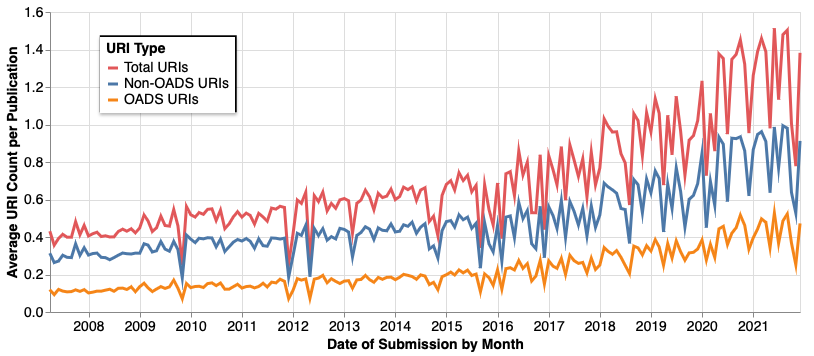
\includegraphics[width=\linewidth]{arxiv_average.png}
    \caption{Average number of URIs per arXiv pre-print by publication date. The blue line represents the number of URIs our machine learning model classified as non-OADS as an average per publication (y-axis) per publication month (x-axis). The orange line represent the number of URIs our machine learning model classified as OADS as an average per publication. The red line represents the total number of URIs we extracted from the publications as an average per publication.}
    \label{fig:arxiv_average}
\end{figure}

With an understanding of the general trends of URI usage, we next looked at the distribution of OADS and non-OADS URIs. We also separated the GHP URIs from the other OADS URIs to gain an understanding of the prevalence of GHP URIs over time. We chose GitHub, GitLab, Bitbucket, and SourceForge as popular GHPs to represent GHP URIs. As shown in Figure \ref{fig:arxiv_percent}, we found that both the prevalence and the distribution of the URIs changed across the time period. The percentage of non-OADS URIs has slightly declined meaning that authors are including a higher proportion of OADS URIs to non-OADS URIs in recent years. The percentage of GHP URIs has significantly increased from less than 1\% in 2007 to around 15\% of all URIs in 2021. Despite the overall increase in the prevalence of OADS URIs seen in Figure \ref{fig:arxiv_average}, there has been a decrease in the percentage of non-GHP OADS URIs as shown in Figure \ref{fig:arxiv_percent}. This means that the growth in the prevalence of OADS URIs has largely been due to an increase in the inclusion of GHP URIs within publications. 

\begin{figure}
    \centering
    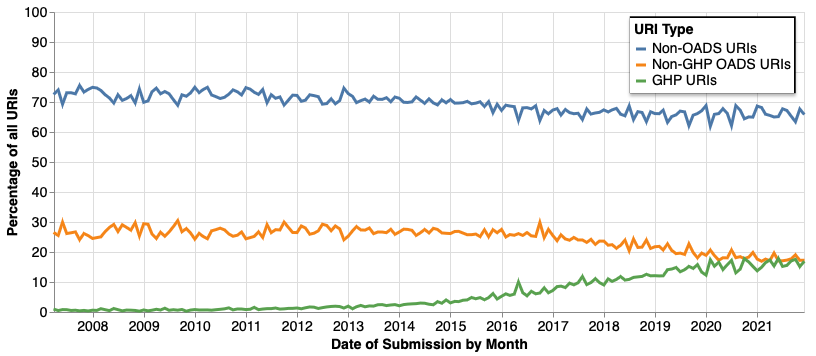
\includegraphics[width=\linewidth]{arxiv_percent.png}
    \caption{Percentage of GHP URIs, non-GHP OADS URIs, and non-OADS URIs by publication date. The blue line represents the percent of URIs our machine learning model classified as non-OADS (y-axis) per publication month (x-axis). The orange line represents the percent of URIs our machine learning model classified as OADS, excluding GHP URIs. The green line represents the percent of URIs that were GHP URIs.}
    \label{fig:arxiv_percent}
\end{figure}

The increase of the prevalence of GHP URIs is also reflected when we look at the total number of GHP and OADS URIs over time in Figure \ref{fig:arxiv_total}. From 2007 to 2015, there were a 500 to 1000 more non-GHP URIs than GHP URIs. In 2015, the number of GHP URIs started to steadily increase. In 2020 and 2021, for every GHP URI, there is a non-GHP OADS URI. This shows that utility of using a classifier to identify OADS URIs, especially in older publications from 2007 to 2015. We also see that, while GitHub is an independently popular GHP, we must look beyond GitHub to identify and discover the full breadth of OADS resources being referenced and produced by researchers even in recent year. 

\begin{figure}
    \centering
    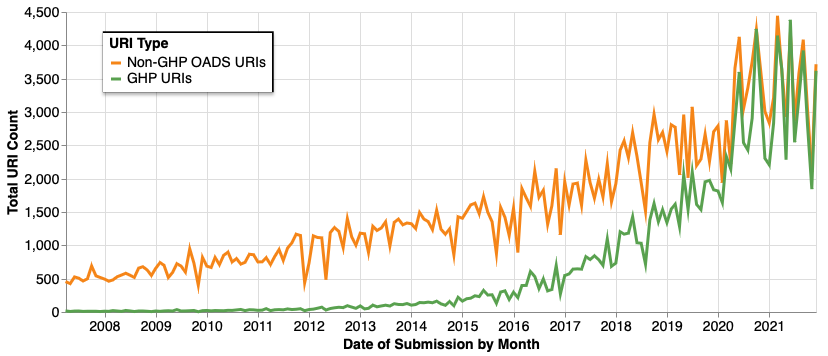
\includegraphics[width=\linewidth]{arxiv_total.png}
    \caption{Total number of GHP URIs and non-GHP OADS URIs by publication date}
    \label{fig:arxiv_total}
\end{figure}

After seeing the trends over time, we wanted to identify the most common non-GHP OADS URIs. We chose to compare URI hostnames and the frequency of those hostnames to determine the most common OADS websites outside of GHPs. In total, we found 258,288 non-GHP OADS URIs included in arXiv publications and almost 50,000 unique hostnames\footnote{The full dataset is available at \url{https://github.com/elescamilla/Extract-URLs/blob/main/classifier\_results/count\_oads\_non\_ghp\_hostnames.csv}} within those URIs. Figure \ref{fig:frequency} shows that 49,392 hostnames are included in between 0 and 50 non-GHP OADS URIs. We found that 63\% of non-GHP OADS URIs are the only URIs to that hostname and only 10\% of URIs reference a hostname that is referenced more than five times. Even with a large number of hostnames referenced a few number of times, there are 19 hostnames that were referenced over 1000 times. Table \ref{tab:hostnames} shows the the top fifteen most common hostnames of non-GHP OADS URIs. However, it is worth noting that the most popular hostname, cds.cern.ch, only accounts for 1.92\% of all non-GHP OADS URIs. Therefore, there are a large number of platforms used by scholars to host data and software which increases the difficulty of archiving data and software products for reproducibility. The diversity of the platforms used and referenced by scholars makes it difficult to manually identify OADS URIs and lends itself to automation like we used with the machine learning classifier model. 

\begin{figure}
    \centering
    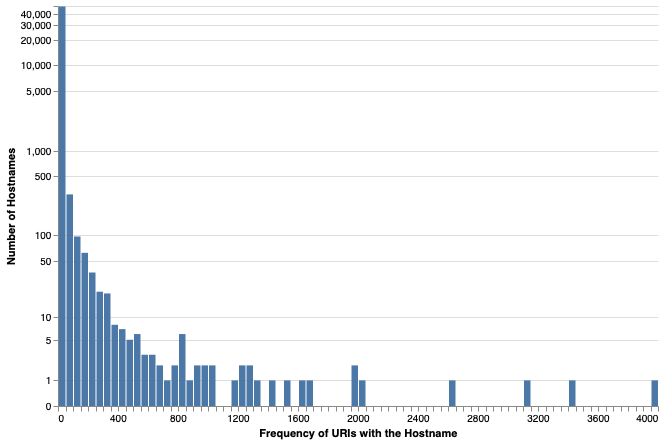
\includegraphics[width=\linewidth]{frequency.png}
    \caption{A histogram showing the frequency of the hostname in non-GHP OADS URIs (x-axis) and the number of hostnames that shared that frequency (y-axis)}
    \label{fig:frequency}
\end{figure}

\begin{table}
    \centering
    \begin{tabular}{|l|c|}
    \hline
    Hostname & Frequency \\
    \hline
    cds.cern.ch & 4,953 \\
    www.sciencedirect.com & 3,119 \\
    archive.ics.uci.edu & 2,632 \\
    adsabs.harvard.edu & 2,031 \\
    www.ncbi.nlm.nih.gov & 1,998 \\
    www.cosmos.esa.int & 1,996 \\
    physics.nist.gov & 1,651 \\
    fermi.gsfc.nasa.gov & 1,627 \\
    heasarc.gsfc.nasa.gov & 1,500 \\
    cran.r-project.org & 1,446 \\
    doi.org & 1,337 \\
    www.w3.org & 1,289 \\
    www.nature.org & 1,275 \\
    archive.stsci.edu & 1,243 \\
    en.wikipedia.org & 1,228 \\
    \hline
    \end{tabular}
    \caption{The top 15 most common hostnames for non-GHP OADS URIs and their frequencies}
    \label{tab:hostnames}
\end{table}